%-------------------------------PPT Title-------------------------------------
\title{\textrm{2024}-职称评审}
%-----------------------------------------------------------------------------

%----------------------------Author & Date------------------------------------
\author[]{姜\;\;骏\inst{}} %[]{} (optional, use only with lots of authors)
% - Give the names in the same order as the appear in the paper.
% - Use the \inst{?} command only if the authors have different
%   affiliation.
\institute[BCC]{\inst{}%
 \vskip -30pt 北京市计算中心\;云平台事业部}
\date[\today] % (optional, should be abbreviation of conference name)
{%	{\fontsize{6.2pt}{4.2pt}\selectfont{\textcolor{blue}{E-mail:~}\url{jiangjun@bcc.ac.cn}}}
\vskip 35 pt \textrm{2024.09.03}
%\vskip 5 pt {\fontsize{8.2pt}{6.2pt}\selectfont{清华大学\;\;材料学院}}
}

% - Either use conference name or its abbreviation
% - Not really information to the audience, more for people (including
%   yourself) who are reading the slides online

%\subject{}
% This is only inserted into the PDF information catalog. Can be left
%\frame
%{	
%	\frametitle{\footnotesize{\textcolor{orange}{\textrm{2018~}年度北京市计算中心职称评聘答辩}}}
%\titlepage
%}
%-----------------------------------------------------------------------------
\maketitle
%------------------------------------------------------------------------------列出全文 outline ---------------------------------------------------------------------------------
\section*{}
%\frame[allowframebreaks]
%{
%  \frametitle{Outline}
%  \frametitle{\textcolor{mycolor}{\secname}}
%  \tableofcontents%[current,currentsection,currentsubsection]
%}
%在每个section之前列出全部Outline
%类似的在每个subsection之前列出全部Outline是\AtBeginSubsection[]
%\AtBeginSection[]
%{
%  \frame<handout:0>
%  {
%    \frametitle{Outline}
%%全部Outline中,本部分加亮
%    \tableofcontents[current,currentsection]
%  }
%}

%------------------------------------------------------------------------------PPT main Body------------------------------------------------------------------------------------
\small
%\section{个人信息}
\frame
{
	\frametitle{个人信息}
	\vskip -35pt
\begin{minipage}[b]{0.72\linewidth}
	\fontsize{9.2pt}{6.2pt}\selectfont{姓~名\hspace{15pt}姜~骏\hspace{45pt}出生年月\hspace{15pt}\textrm{1978.12}}\\
	\vskip 7pt
	学~位\hspace{15pt}理学博士\hspace{29pt}专业方向\hspace{15pt}物理化学\\
	\vskip 7pt
	\fontsize{8.2pt}{6.2pt}\selectfont{工作部门\hspace{5pt}北京市计算中心~云平台事业部}\\
\end{minipage}
\hfill
\begin{minipage}[b]{0.26\linewidth}
	\vspace{40pt}
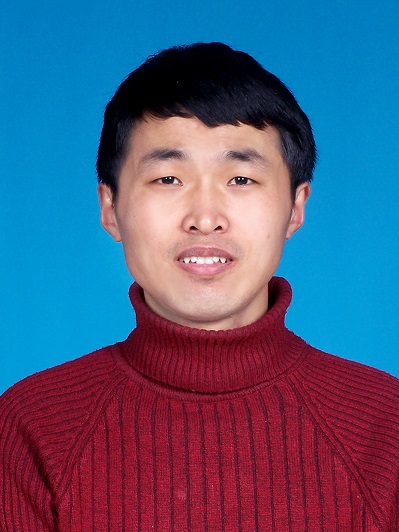
\includegraphics[height=0.7in]{Figures/Person_Photo.JPG}
\end{minipage}\vskip 3pt
\fontsize{9.2pt}{6.2pt}\selectfont{\textcolor{magenta}{教育背景}}
	\begin{itemize}
		\item {\fontsize{8.2pt}{6.2pt}\selectfont{\textrm{2001.09-2008.01}}}~~~北京大学~化学与分子工程学院~~~~~~物理化学
		\item {\fontsize{8.2pt}{6.2pt}\selectfont{\textrm{1997.09-2001.06}}}~{\fontsize{8.2pt}{6.2pt}\selectfont{中国纺织大学(现~东华大学)}}~{\fontsize{8.2pt}{6.2pt}\selectfont{纺织化学系~染整工程}}
	\end{itemize}
	\fontsize{9.2pt}{6.2pt}\selectfont{\textcolor{magenta}{工作简历}}
\begin{minipage}{\textwidth}
\begin{table}[!h]
\tabcolsep 0pt %\vspace*{-5pt}
%\caption{经费预算表 (单位:~万元).}
\label{Table-Cost}
%\begin{center}
\centering
\def\temptablewidth{0.94\textwidth}
\renewcommand\arraystretch{2.2} %表格宽度控制(普通表格宽度的两倍)
\rule{\temptablewidth}{1pt}
\begin{tabular*} {\temptablewidth}{@{\extracolsep{\fill}}c@{\extracolsep{\fill}}c@{\extracolsep{\fill}}c}
%-------------------------------------------------------------------------------------------------------------------------
	起止时间 &工作单位	&研发岗位 \\\hline
	\fontsize{8.2pt}{6.2pt}\selectfont{\textrm{2008.01-2012.03}} &\fontsize{8.2pt}{6.2pt}\selectfont{北京大学~化学与分子工程学院} &\fontsize{8.2pt}{6.2pt}\selectfont{博士后} \\
	\fontsize{8.2pt}{6.2pt}\selectfont{\textrm{2012.03-2013.03}} &\fontsize{8.2pt}{6.2pt}\selectfont{北京宏剑公司} &\fontsize{8.2pt}{6.2pt}\selectfont{高级技术支持}\\
	\fontsize{8.2pt}{6.2pt}\selectfont{\textrm{2013.04-2016.03}} &\fontsize{7.8pt}{6.2pt}\selectfont{中物院高性能数值模拟软件中心} &\fontsize{8.2pt}{6.2pt}\selectfont{金属材料模拟团队} \\
	\fontsize{8.2pt}{6.2pt}\selectfont{\textrm{2016.04-至今}}    &\fontsize{8.2pt}{6.2pt}\selectfont{北京市计算中心} &\fontsize{8.2pt}{6.2pt}\selectfont{云平台事业部}\\
\end{tabular*}
\rule{\temptablewidth}{1pt}
%\end{center}
\end{table}
%\vskip -3pt
\end{minipage}
}

\begin{frame}
	\frametitle{承担项目}
\begin{itemize}
	\setlength{\itemsep}{5pt}
	\item {\fontsize{8.2pt}{6.2pt}\selectfont{国家重点研发计划项目~(本单位任务责任人~\textcolor{red}{已结题})}}
		\vskip 2pt
		“高通量并发式材料计算算法和软件”
		\vskip 2pt
		{\fontsize{8.2pt}{4.2pt}\selectfont{项目编号:~\textrm{2017YFB0701500}}}
		\vskip 1pt
		{\fontsize{8.2pt}{6.2pt}\selectfont{执行时间:~\textrm{2017.07-2021.06}}}
	\item {\fontsize{8.2pt}{6.2pt}\selectfont{北科院青年骨干计划项目}}{\fontsize{8.2pt}{4.2pt}\selectfont{(项目负责人~\textcolor{red}{已结题})}}
		\vskip 2pt
“基于甲烷催化燃烧机理的材料计算自动流程设计”
		\vskip 2pt
		{\fontsize{8.2pt}{4.2pt}\selectfont{项目编号:~\textrm{YC201820}}}
		\vskip 1pt
		{\fontsize{8.2pt}{6.2pt}\selectfont{执行时间:~\textrm{2018.01-2019.12}}}
	\item {\fontsize{8.2pt}{6.2pt}\selectfont{国家自然科学基金~(本单位项目责任人)}}
		\vskip 2pt
“低维材料等离和激子极化激元的第一性原理研究”
\vskip 2pt
		{\fontsize{8.2pt}{4.2pt}\selectfont{(项目批准号:~\textrm{12474217})}}
		\vskip 1pt
		{\fontsize{8.2pt}{6.2pt}\selectfont{(项目持续年度:~ \textrm{2025.01-2028.12})}}
\end{itemize}
\end{frame}

\begin{frame}
	\frametitle{发表论文}
	\begin{itemize}
		\item {\fontsize{5.2pt}{1.2pt}\selectfont{\textrm{Zhenxi Pan, Yong Pan, \underline{Jun Jiang} and Liutao Zhao$^{\dagger}$, \textcolor{blue}{High-Throughput Electronic Band Structure Calculations for Hexaborides}, \textit{CompCom~2019 AIOSC}, \textbf{998}, (2019), 386-395}}}
		\item {\fontsize{5.2pt}{1.2pt}\selectfont{\textrm{Yurui Wang, Zhihui Du$^{\dagger}$, \underline{Jun Jiang}, Baokun Lu and Chongyu Wang, \textcolor{blue}{Modeling the Parallel Efficiency of Density Functional Theory based Jobs on Sunway TaihuLight}, \textit{2019 IEEE-CSE and IEEE-EUC}, (2019), 199-204}}}
		\item {\fontsize{5.2pt}{1.2pt}\selectfont{\textrm{Zhihui Du$^{\dagger}$, Xinning Hui, Yurui Wang, \underline{Jun Jiang}, Jason Liu, Baokun Lu and Chongyu Wang, \textcolor{blue}{Inter-Job Scheduling of High-Througput Material Screening Applications}, \textit{2020 IPDPS}, (2020), 841-852}}}
		\item {\fontsize{5.2pt}{1.2pt}\selectfont{\textrm{Jianxin Huang, Jinkai Wang, Hao Wang$^{\dagger}$, Jiajun Lu, Xiao-Gang Lu, \underline{Jun Jiang} and Ying Chen, \textcolor{blue}{Influences of multicenter bonding and interstitial elements on psudo-twinned $\gamma$-\ch{TiAl} crystal}, \textit{Phys. Scr.}, \textbf{97}, (2022), 085403}}}
		\item {\fontsize{5.2pt}{1.2pt}\selectfont{\textrm{Caiqun Wang, Penglin Gao, Hongfei Li, Mei Yang, \underline{Jun Jiang}, Liutao and Ping Qian$^{\dagger}$, \textcolor{blue}{Single-atom catalysts:~Effects of end-group regulation on catalytic activity}, \textit{Mater. Tod. Comm..}, \textbf{40}, (2024), 109482}}}
	\end{itemize}
\end{frame}
%\section{第一原理材料计算核心软件研究}
\frame
{
	\frametitle{著作}
\begin{itemize}
%	\setlength{\itemsep}{1pt}
	\item {\fontsize{8.0pt}{4.2pt}\selectfont{赵琉涛, \underline{姜骏}, 王彩群, 潘勇, 潘震西, \textcolor{blue}{计算材料科学理论与实践}, 人民邮电出版社, (北京), 2021}}
\end{itemize}
\begin{figure}[h!]
\centering
\vskip -5pt
\includegraphics[height=2.3in,width=1.6in]{/home/jun-jiang/BCC/年度工作/03-著作-封面.jpg}
\label{Fig:Cover}
%\caption{\fontsize{5.2pt}{6.2pt}\selectfont{$\vec k\cdot\vec p$方法保证计算精度,并计算效率提升}}%
\end{figure}
}

\frame
{
	\frametitle{专利}
	\begin{itemize}
		\item {\fontsize{7.5pt}{6.2pt}\selectfont{\underline{姜骏}, 王崇愚, 晶体对称性及能带路径确定方法及装置}}
	\end{itemize}
\begin{figure}[h!]
\centering
\vskip -5pt
\includegraphics[height=2.3in,width=1.6in]{/home/jun-jiang/BCC/年度工作/05-专利.png}
\label{Fig:Patent}
%\caption{\fontsize{5.2pt}{6.2pt}\selectfont{$\vec k\cdot\vec p$方法保证计算精度,并计算效率提升}}%
\end{figure}
}

\begin{frame}
	\frametitle{效益产出}
	\begin{itemize}
		\item {\fontsize{7.5pt}{6.2pt}\selectfont{一种超融合混合架构计算材料平台,~\textrm{2024}}}
	\end{itemize}
\begin{figure}[h!]
\centering
\vskip -5pt
\includegraphics[height=2.1in,width=1.7in]{/home/jun-jiang/Pictures/Screenshot from 2024-09-04 11-43-06.png}
\includegraphics[height=2.1in,width=2.1in]{/home/jun-jiang/Pictures/Screenshot from 2024-09-04 11-43-15.png}
\label{Fig:Contract}
%\caption{\fontsize{5.2pt}{6.2pt}\selectfont{$\vec k\cdot\vec p$方法保证计算精度,并计算效率提升}}%
\end{figure}
{\fontsize{7.5pt}{6.2pt}\selectfont{另有两份合同盖章未返回,直接收益合计约\textrm{36}万元}}
\end{frame}
%\section{高通量材料计算自动流程软件开发}
\begin{frame}
	\frametitle{其它奖励}
\begin{figure}[h!]
\centering
\vskip -5pt
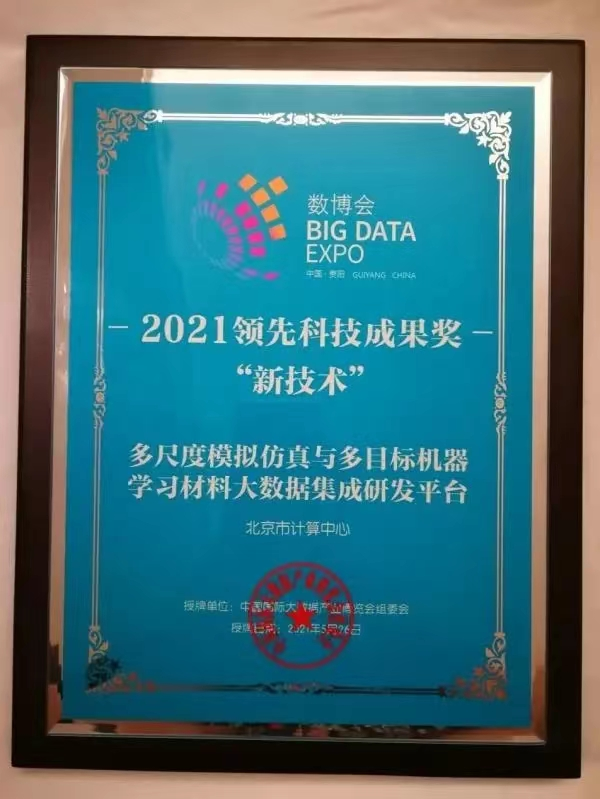
\includegraphics[height=2.5in,width=1.9in]{/home/jun-jiang/BCC/Report_Papers_Awards/2021-BigData_Expo.jpg}
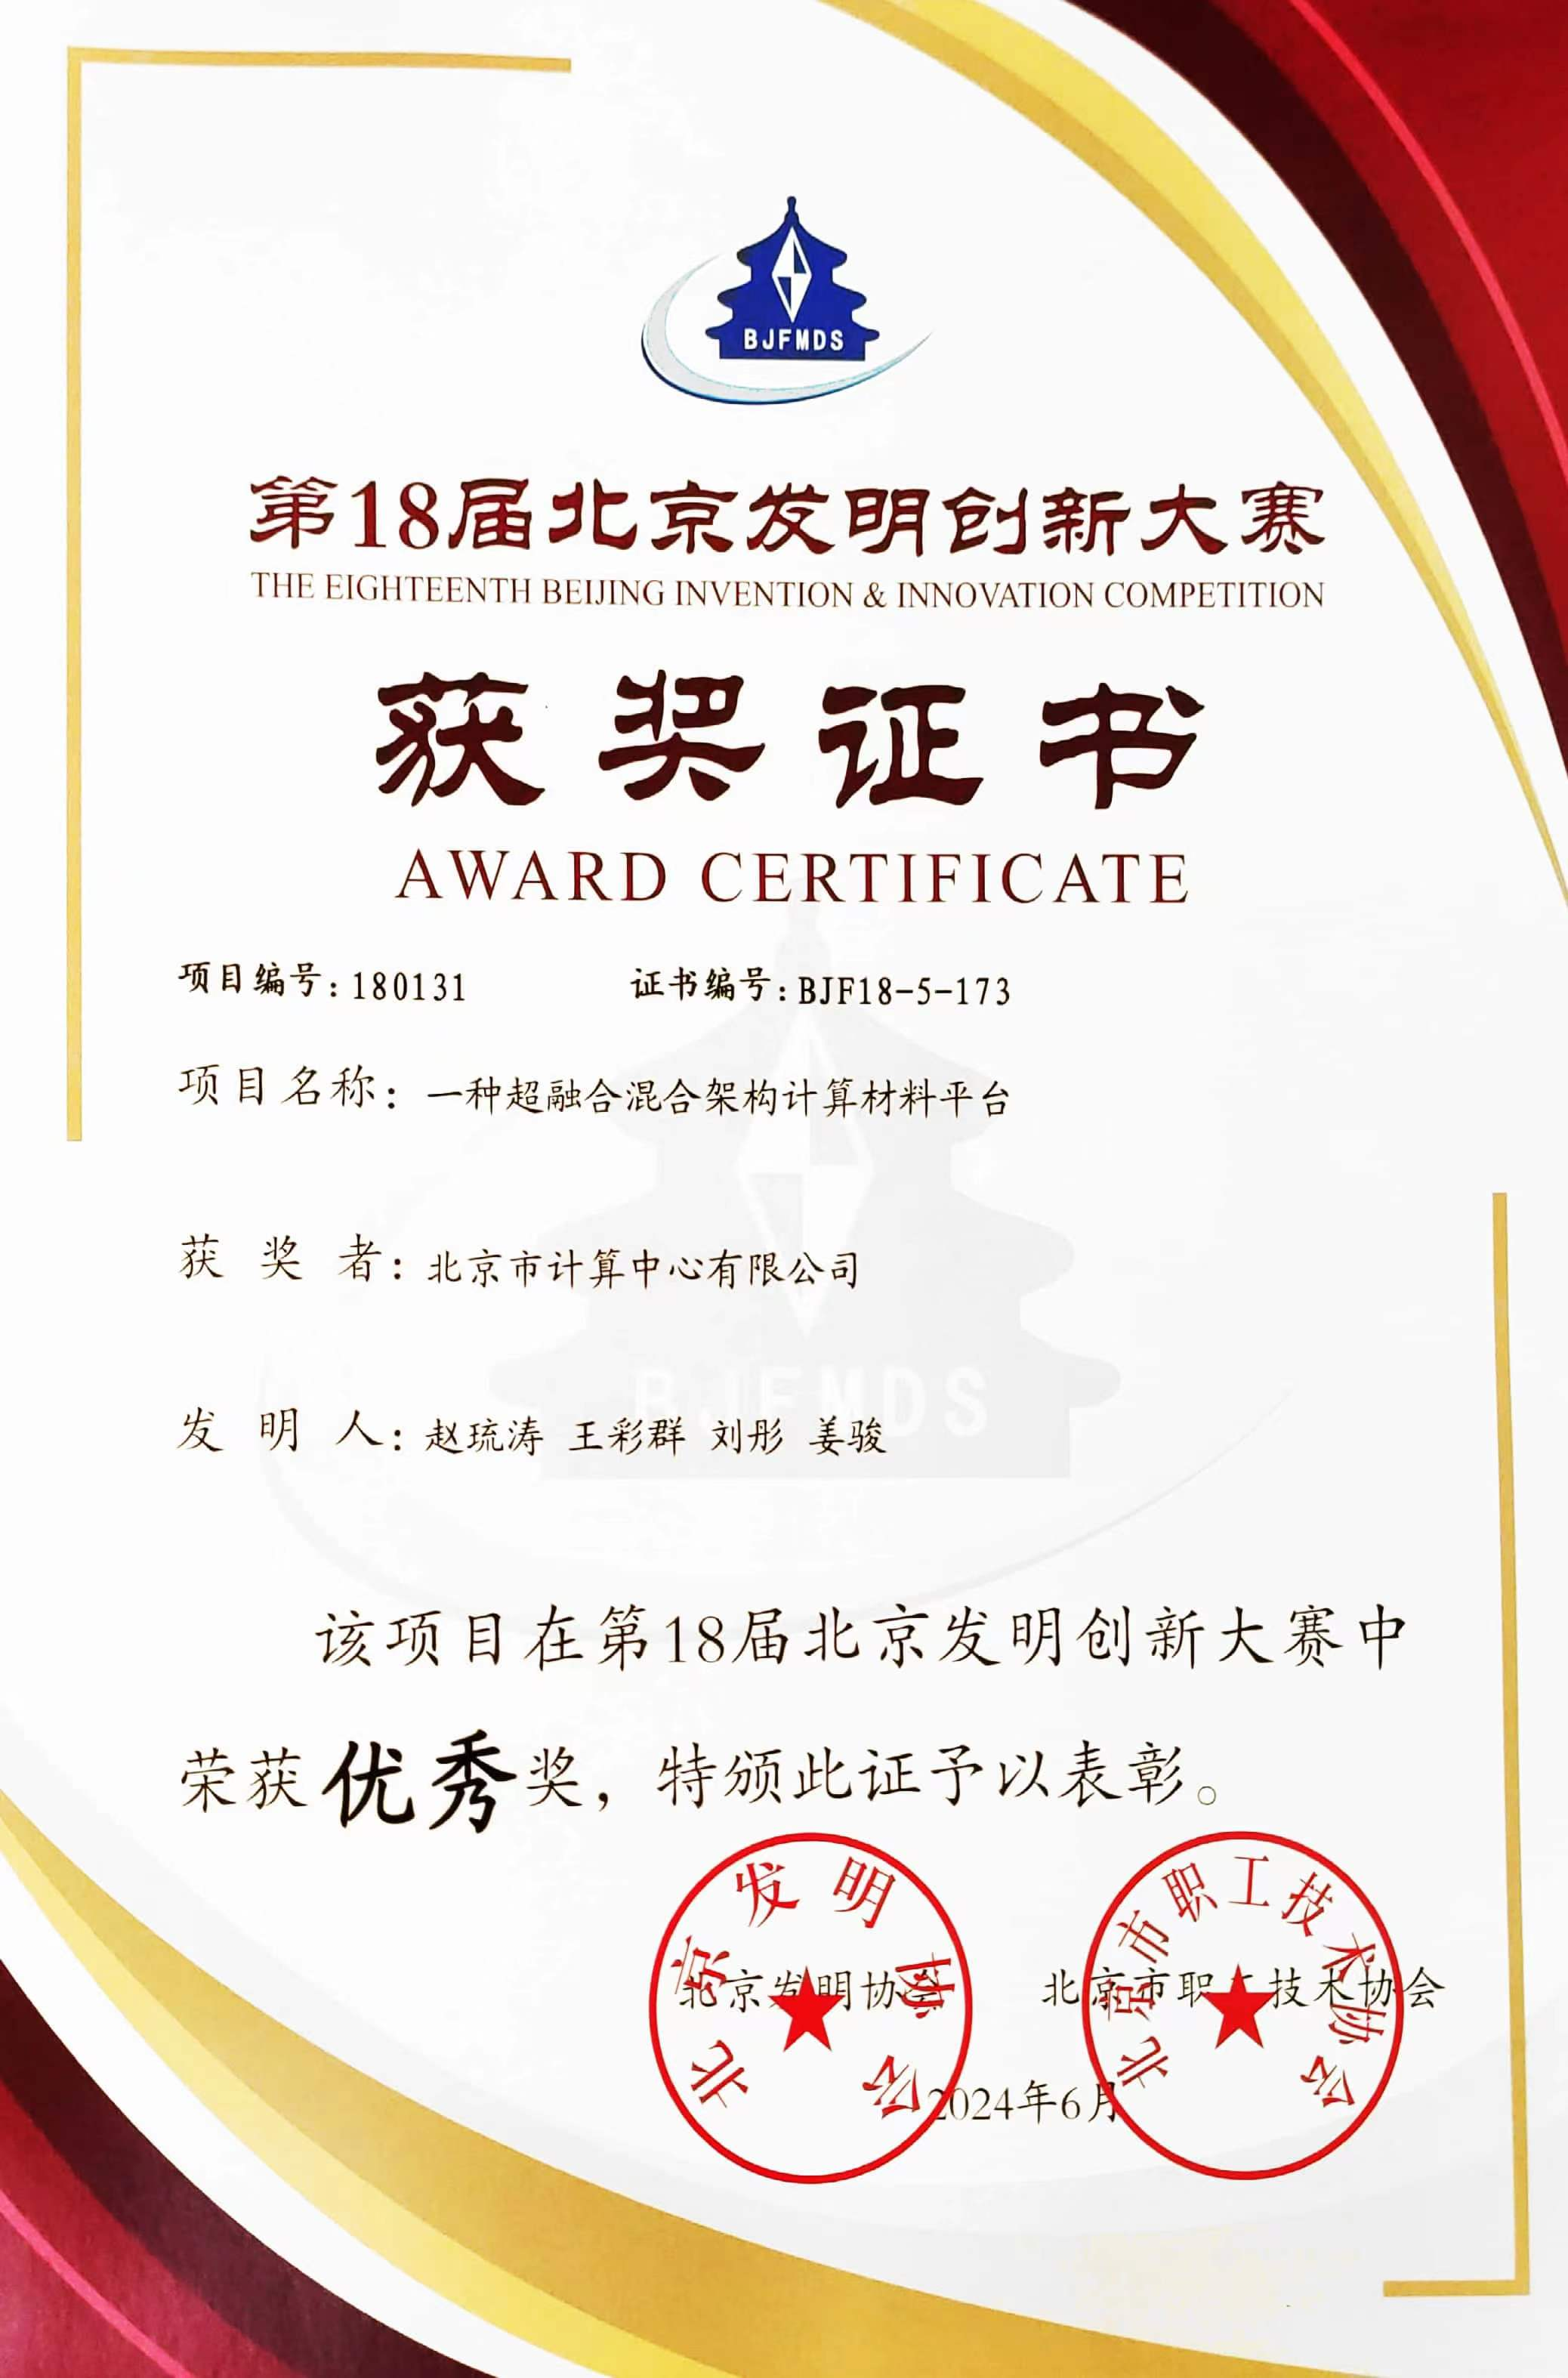
\includegraphics[height=2.5in,width=1.9in]{/home/jun-jiang/BCC/Report_Papers_Awards/2024-Innovation.jpg}
\label{Fig:Award}
%\caption{\fontsize{5.2pt}{6.2pt}\selectfont{$\vec k\cdot\vec p$方法保证计算精度,并计算效率提升}}%
\end{figure}
\end{frame}

\frame
{
	\frametitle{社会影响}
	\begin{itemize}
		\setlength{\itemsep}{15pt}
		\item 多次组织和主讲“第一原理材料计算方法与软件”培训,课程面向高校物理、化学与材料专业的研究生和教师
		\item 防疫期间\textrm{(2020-2022)},在线讲授第一原理材料计算基础理论、计算方法、程序算法和软件结构,主要包括:\vskip 5pt
			{\fontsize{8.5pt}{4.2pt}\selectfont{密度泛函基本理论、固体能带理论}}\vskip 5pt
			{\fontsize{8.5pt}{4.2pt}\selectfont{赝势-平面波方法、\textrm{LAPW~}方法、\textrm{LMTO~}方法、\textrm{PAW~}方法}}\vskip 5pt
			{\fontsize{8.5pt}{4.2pt}\selectfont{$\vec k$-空间积分方法、电子相关与磁性(\textrm{LDA+$U$}方法)}}\vskip 5pt
			{\fontsize{8.5pt}{4.2pt}\selectfont{\textrm{WIEN2k}/\textrm{ELK}/{\textrm{VASP}/\textrm{ABINIT}等软件结构与使用}}}
		\item \textrm{2021.10},受中科院理论物理所邀请,参加中科院学部咨询评议项目支持的“我国科学计算软件的现状、问题及对策研讨会”并作学术报告
	\end{itemize}
}

%\appendix
%\frame
%{
%	\frametitle{学术积累}
%\textcolor{magenta}{发表论文}
%	\begin{itemize}
%		\item {\fontsize{5.2pt}{1.2pt}\selectfont{\textrm{Yang Ge, Jianlong Ji, Zhizhong Shen, Qiang Zhang, Aoqun Jian, Qianqian Duan, Chao Wang, \underline{Jun Jiang}, Wendong Zhang, Shengbo Sang, First principles study of magnetism induced by topological frustration of bowtieshaped graphene nanoflake, \textit{Carbon}, \textbf{127}, (2018), 432-436}}}
%		\item {\fontsize{5.2pt}{1.2pt}\selectfont{\textrm{\underline{JIANG Jun}, BIAN Jiang; LI Le-Min, Theoretical Assignments of the Optical Conductivity and Energy-loss Function Spectra of EuB$_6$, \textit{Acta Physico-Chimica Sinica}, \textbf{24}, (2008), 1-7}}}
%	\end{itemize}
%}
